\documentclass[11pt]{article}

% ---------- Layout (matches v3.5) ----------
\usepackage[letterpaper,margin=1.05in]{geometry}
\usepackage{mathptmx}
\usepackage[T1]{fontenc}
\usepackage{amsmath,amssymb}
\usepackage{enumitem}
\usepackage{booktabs}
\usepackage{array}
\usepackage{longtable}
\usepackage{graphicx}
\usepackage{tikz}
\usetikzlibrary{arrows.meta,positioning,calc}
\usepackage{titlesec}
\usepackage{fancyhdr}
\usepackage[hidelinks,colorlinks=false,pdfborder={0 0 0}]{hyperref}
\usepackage{caption}
\usepackage{xcolor}

\titleformat{\section}{\normalfont\bfseries\large}{\thesection.}{0.6em}{}
\titleformat{\subsection}{\normalfont\bfseries}{\thesubsection}{0.6em}{}
\titlespacing*{\section}{0pt}{1.6ex plus 1ex minus .2ex}{1ex}
\titlespacing*{\subsection}{0pt}{1.3ex plus .8ex minus .2ex}{0.6ex}
\setlength{\parindent}{1.4em}\setlength{\parskip}{0pt}
\renewcommand{\headrulewidth}{0.4pt}\pagestyle{fancy}\fancyhf{}
\fancyhead[L]{\small\scshape Fenn \& Fenn}
\fancyhead[R]{\small\scshape Evolution as Active Geometry}
\fancyfoot[C]{\small\thepage}
\captionsetup{font=small,labelfont=bf,justification=raggedright,singlelinecheck=false}

\newcommand{\hpack}{h_{\mathrm{pack}}}
\newcommand{\heff}{h_{\mathrm{eff}}}
\newcommand{\Crel}{C_{\mathrm{rel}}}
\newcommand{\Cblock}{C_{\mathrm{block}}}
\newcommand{\Hk}{\mathbb{H}^n_\kappa}
\newcommand{\Htwo}{\mathbb{H}^2}

\begin{document}
\thispagestyle{empty}

\begin{center}
{\LARGE\bfseries Evolution as Active Geometry}\\[4pt]
{\Large\bfseries Descent Under the Addressability Limit}\\[16pt]
{\large Rohit Fenn\textsuperscript{1}\ \ and\ \ Amit Fenn\textsuperscript{1}}\\[4pt]
{\small\textsuperscript{1}Sentry Bio, Inc., USA}\\[2pt]
{\small Correspondence: \texttt{research@sentry.bio}}\\[2pt]
{\small\itshape Version Gf --- 15 October 2026}
\end{center}

\vspace{6pt}\noindent\rule{\textwidth}{0.4pt}\vspace{4pt}

\footnotesize
\noindent\textbf{On this version.} A companion paper, \emph{The Addressability Limit} (Paper~I), proves a ceiling on how much distinguishable history a process can retain in a given amount of representational room, a ladder separating bare identity from preserved genealogy, and an identity that factors a medium's efficiency into five losses. This paper asks what descent, and the genome that records it, do underneath that ceiling; it carries the limit, the ladder, the audit and the random writer's window as cited results and re-derives none. Two earlier versions are retired by name. The bioRxiv version (2026.03.09.710612v2) reported a curvature--entropy ``state equation'' read off the object it was meant to explain (Appendix~A); the August version (v3.5) led with the claim that descent \emph{measurably} occupies exponential room, from a metric that proved polynomial in growth (\S2). What survives both retirements is stronger for being narrower: the two prices of heredity, the window inside which a random writer keeps its past, and the audit of where each real medium loses it. This version adds the one inequality that runs through both papers (\S1), four registered tests of 14 October (PREREG22--24, Appendix~C), and withdraws the two-bit ceiling comparison as a units error (\S4). Every number below traces to a registration written before its data were read.\normalsize

\vspace{6pt}
\noindent\textbf{Abstract.}
A newly arising lineage must be given an identity that collides with no other, and connected by a path to the parent it descended from. These are two different demands---an address, and a route between addresses---and a companion paper proves that any process meeting them lives under a ceiling: it cannot retain distinguishable histories faster than its representation gains room to hold them apart. Here we ask what descent does under that ceiling and what a genome preserves of it. The room almost never binds; timing does. Identity is kept cheaply, at a cost logarithmic in the number of lineages that falls as substitution rises. Genealogy is kept expensively, and only inside a window: ancestry stays readable while the sampled tree branches faster than twice the rate at which the carrying sites forget. On a registered harness the price of genealogy changes class across that line within 3\% of a parameter-free prediction, the ratio of the two prices holds within 7\%, and a composition reader is worth one to two aligned sites whatever the genome length. Genealogy fails in two distinguishable ways---quietly, when a finite tape is overwritten at depth and more sequence repairs it, or wrongly, when a second history competes for the tape---and block structure of the wrong quartets separates the second from model misspecification. The audit of a medium's losses closes on an engineered cellular recorder in states and fails in information, where the reading anomaly proves to be the measure. Readable depth grows as the logarithm of the record at one rate and as a power of it under a slow rate tail, the law that governs synaptic memory. On vertebrate mitogenomes its finite-length prediction holds with no free parameter to 512 sites and the rate-weighted reader's advantage is confirmed; the depth exponents are blocked by a reader-dependent floor, sitting on short internal edges, that more sequence does not remove. No medium measured approaches its ceiling.

\vspace{4pt}
\noindent{\small\itshape\sloppy Keywords: phylogenetics; horizontal gene transfer; information capacity; Kesten--Stigum threshold; lineage recorders; alignment-free methods; addressability\par}

\vspace{8pt}\noindent\rule{\textwidth}{0.4pt}
\bigskip

% =====================================================================
\section{The limit, and how to read this paper}
% =====================================================================

Every newly arising lineage needs two things that are easy to confuse and, it turns out, are kept in different places. It needs an \emph{identity}: a state distinguishable from every other lineage alive, so that it can be named without collision. And it needs a \emph{record of descent}: a path back through its ancestry, so that its relationships can be recovered. The first is an address. The second is a route between addresses. A genome carries both, and this paper is about how differently it holds them.

Cast formally, this is an addressing problem in a metric space, and a companion paper proves the constraint that governs it. One inequality runs through both papers: histories that are far apart must stay far apart in the record, $D^{-1}d_S(u,v)-K\le d_M(\mathrm{addr}\,u,\mathrm{addr}\,v)$, which at the distance of sisters is the resolution condition that gives identity and at the distance of deep cousins is the condition that keeps genealogy. The companion asks which hosts can honour it at exponential rate; this paper asks how long a random writer honours it, and what a bounded reader recovers. Every failure reported below is a failure of that one inequality at some depth. We import five of the companion's results and re-derive none.

\begin{description}[leftmargin=1.2em,style=nextline]
\item[The room (the limit).] A process that retains distinguishable histories at exponential rate $\beta$, addressed at a finite rate $c$ into a host whose room grows at packing rate $\hpack$, obeys $\beta \le c\,\hpack$. At a single depth the bound is a minimum of two counts: the number of lineages a reader of resolution $\varepsilon$ can distinguish is at most the smaller of the number of lineages and the number of $\varepsilon$-separated states the room holds. Read as a fork: a process that keeps its history either occupies a host with \emph{exponential} room, or its addresses outrun any finite budget, or it is forgetting. This is a theorem about any process that remembers. It is not, in this paper, a measurement.
\item[Names versus paths (the ladder).] Holding distinguishable \emph{endpoints} (identity) and preserving the \emph{genealogy} that connects them (descent) are different achievements. The second can cost more than the first, and a representation can pay the first in full while defaulting on the second. (Paper~I shows that the intermediate rung---one nested family of addresses that never move---costs nothing in a host of bounded geometry; the price, where there is one, is paid when paths must be preserved.)
\item[The audit.] Efficiency against the ceiling is a product of five ratios, each at most one---availability, writing, retention, collisions, reading---and the identity's whole content is the experiment that estimates each from its own mechanism and checks that the product closes.
\item[The classifier (quartets).] A distance matrix is an exact tree exactly when, for every four taxa, the two larger of the three pairwise-sum pairings agree (Buneman 1971). The residual, quartet defect $\delta$, measures departure from a tree. It is independent of how much room the data occupy, and it does not determine growth class.
\item[The window (finite tapes).] On a tape of $L$ letters written by a random process at rate $\rho$, a distance reader's identity edge is one-sided (faster never hurts) and its genealogy edges bound $\rho$ in an explicit interval: too slow and the internal branch is unwritten, too fast and the deep contrast saturates, with readable depth at most $\log(3\sqrt L/4\kappa)/2\rho$ at one rate. Both edges are the one inequality at two depths; the Kesten--Stigum line is the same inequality for a census reader whose resolution sharpens with the clade (\S5.4), and only the optimal reader on large alphabets escapes it.
\end{description}

\noindent\textbf{What kind of statement this is.} The bound is a ceiling in the sense Shannon's capacity is a ceiling: it cannot be beaten, and reaching it is a design act. Coded transmission approaches capacity; uncoded transmission sits far below it. Heredity, we will find, is uncoded. We use the ceiling to say what descent must do; we never claim life sits at it, and every efficiency we measure says it does not.

\medskip
\noindent\textbf{The compass: the room and the tape.} One distinction runs through every section. The \emph{room} is the process of descent itself---the branching history being addressed. The \emph{tape} is the genome, the finite four-letter record that encodes that history after the fact. These are not the same object, and the central error of the first version of this paper was to read a property of the room (its curvature) directly off the tape. Whenever a measurement appears below, the first question to ask is which of the two it is measuring. A third object joins them here: the \emph{reader}, the procedure that turns a record into a genealogy. The reader turns out to matter as much as the medium.

\medskip
\noindent\textbf{Instruments that can refuse, and registrations that can fail.} Every claim here rests on an instrument able to return \emph{no signal} when there is none to find, and on a registration written before its data were read, with decision rules fixed in advance. Of the two dozen registrations in this program, roughly half failed as registered, and the failures are reported as failures (Appendix~C). A frame that has never failed a pre-registered test has never been tested.

\medskip
\noindent\textbf{Where this sits in the theory of heredity.} Maynard Smith and Szathmáry's distinction between limited and unlimited heredity is a statement about heredity's forward face: how many types a carrier can hold for selection to choose among, measured against population size, with template replicators at $a^L$ types against an ensemble's polynomial count (Maynard Smith and Szathmáry 1995; Szathmáry 2000). This paper is about the backward face: how much of a lineage's past its present record still carries, and what a bounded reader recovers of it. The two are not the same quantity, and one frame holds both. The room count is Szathmáry's, machine-checked and extended to every fixed-window statistic (\S3.3); what is new is the genealogical counterpart of unlimited heredity, the price of keeping ancestry rather than identity, the window inside which a random writer keeps it, and the reader as a locus of limitation in its own right. Where the forward and backward faces must agree, and where they come apart, is the subject of \S5.4.

\subsection{What this paper claims, by layer}

\begin{center}\small
\begin{tabular}{@{}>{\raggedright\arraybackslash}p{5.6cm}>{\raggedright\arraybackslash}p{1.8cm}>{\raggedright\arraybackslash}p{5.6cm}@{}}
\toprule
\textbf{Finding} & \textbf{Layer} & \textbf{Stated as} \\
\midrule
Descent that remembers occupies exponential room & I & Consequence of the theorem; \emph{not measured}. The functional metric is polynomial in growth (\S2) \\
Identity is cheap, genealogy is dear, and the price of genealogy changes class at the line $\beta=2\rho$ (\S3) & I / ladder & Measured on the harness within 3\% and 7\% of parameter-free prediction; the line is Kesten--Stigum's \\
A composition reader is worth one to two aligned sites, independent of genome length (\S3) & reader & Predicted in closed form, confirmed on new seeds within 3 SE \\
Poverty and mixing are distinct exits; a floor alone is not specific; block structure is (\S3) & I / ladder & Certified on synthetic ground truth; the specific diagnostic is two-part \\
The audit closes on a recorder in states once correlated writing is named, and fails in information: the count-based reading anomaly was the measure; the real colonies carry lineage-specific activity the writer does not place (\S4) & audit & Measured on both splits; $\eta=0.12$--$0.20$ in states, $0.04$--$0.09$ in information; information closure failed as registered (PREREG24) \\
Readable depth: $\ln L$ at one rate, a power of $L$ under a slow rate tail, with a reader-dependent exponent (\S5) & law-shaped & Exact finite-$L$ curves, confirmed in simulation (PREREG22); on real mitogenomes the finite-$L$ prediction and the reader ordering hold with no free parameter, and the exponents are blocked by a reader-dependent floor (PREREG23, 23b) \\
A hyperbolic host \emph{specifically}; the process saturates its room & IIa, IIb & Open; not claimed. Every measured $\eta$ is far below one \\
Sequence-tree curvature $=(h\ln2)^2$ & retired & Withdrawn (Appendix~A) \\
\bottomrule
\end{tabular}
\end{center}

% =====================================================================
\section{The room: what the theorem says, and what the data did not}
% =====================================================================

The governing figure of this paper has two axes---how fast a representation's room grows (its growth class), and how far the data depart from a tree (quartet defect $\delta$)---and a silent third coordinate: whether the object plotted is the room, the tape, or a reader's image of the tape.

The theorem settles the first axis for the room itself: a process that retains exponentially accumulating lineages occupies exponential room, on pain of forgetting or of an address budget that never settles (Paper~I, Corollary~2.7). Descent remembers; so descent occupies exponential room. That is a deduction, and we state it as one.

The August version of this paper tried to \emph{measure} it. KEGG ortholog profiles (Kanehisa and Goto 2000) across $1{,}935$ genomes spanning the three domains---a representation built without any geometric model and without sequence distance---give a four-point defect ratio of $0.32$ against a dimension-matched Euclidean null: markedly more tree-like than the best flat arrangement of the same data. We reproduce that number exactly ($0.323$) on the same sample, which is the stratified draw of at most 120 genomes per phylum from a $29{,}303$-genome panel. It is a classifier-level fact and it survives. But v3.5 named the growth-class gate as the single run that would graduate it to a certified measurement of the room, and stated the kill line: the metric is certified polynomial against a matched null. That run was registered and executed (PREREG18). From 25 centres, 21 read polynomial and one exponential, while the matched Gaussian null read polynomial from 24; a second, random sample of the same size read 18 polynomial and 5 exponential. Ball occupancy in the pathway metric grows as a power of the radius, with exponent between two and four. The kill line fired.

This is what Paper~I's bridge section says it can be: the four-point condition decides tree-likeness, not growth class, and an $868$-coordinate pathway profile is a bounded reader's image of a genome (\S3), which can be polynomial for an exponential process. That is the reading the theorem licenses, not a rescue of the measurement: v3.5 claimed exponential room had been \emph{seen}, and it has not been. Where exponential growth could be certified in a real representation of descent is an open instrument question (the Atlas base map of \S5, a composition, is not a candidate). The rest of the paper turns to the tape and the reader, where the measurements are.

\begin{figure}[t]
\centering
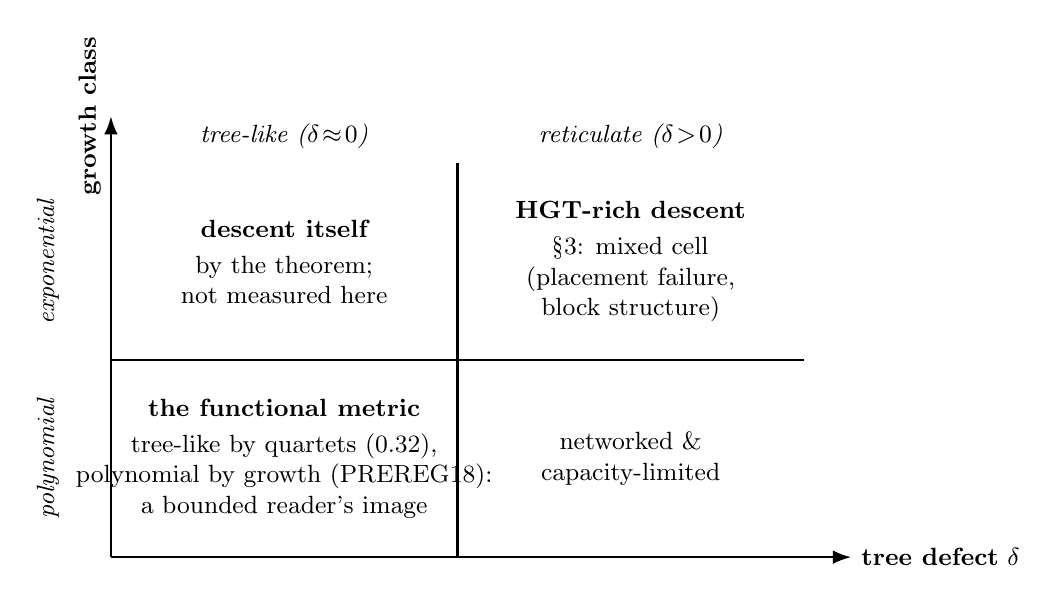
\begin{tikzpicture}[scale=1.0,every node/.style={font=\small}]
  \def\x{4.4}\def\y{2.5}
  \draw[thick,-Latex] (0,0) -- (0,2*\y+0.6) node[above,rotate=90,anchor=south] {\textbf{growth class}};
  \draw[thick,-Latex] (0,0) -- (2*\x+0.6,0) node[right] {\textbf{tree defect} $\delta$};
  \draw[thick] (0,\y) -- (2*\x,\y);\draw[thick] (\x,0) -- (\x,2*\y);
  \node at (\x/2,2*\y+0.35) {\itshape tree-like ($\delta\!\approx\!0$)};
  \node at (\x+\x/2,2*\y+0.35) {\itshape reticulate ($\delta\!>\!0$)};
  \node[rotate=90] at (-0.8,1.5*\y) {\itshape exponential};
  \node[rotate=90] at (-0.8,0.5*\y) {\itshape polynomial};
  \node[align=center] at (\x/2,1.5*\y) {\bfseries descent itself\\[2pt]\small by the theorem;\\ not measured here};
  \node[align=center] at (\x+\x/2,1.5*\y) {\bfseries HGT-rich descent\\[2pt]\small \S3: mixed cell\\ (placement failure,\\ block structure)};
  \node[align=center] at (\x/2,0.5*\y) {\small \bfseries the functional metric\\[2pt]\small tree-like by quartets (0.32),\\ polynomial by growth (PREREG18):\\ a bounded reader's image};
  \node[align=center] at (\x+\x/2,0.5*\y) {\small networked \&\\ capacity-limited};
\end{tikzpicture}
\caption{The governing figure, corrected. Growth class against tree defect. The room descent occupies sits in the upper-left cell by the theorem. The KEGG functional metric, which v3.5 placed there at classifier strength, sits in the lower-left: tree-like by the four-point condition and polynomial by ball growth, as a bounded reader's image of an exponential process can be. Sections~3--4 characterize how a sequence tape leaves the upper-left cell---apparently, under poverty, or really, under mixing.}
\end{figure}

% =====================================================================
\section{Identity is cheap; ancestry is dear}
% =====================================================================

The ladder says identity---distinguishable endpoints---and genealogy---the preserved path between them---are different capacities. Biologically, this is the difference between telling two organisms apart and reconstructing how they are related. This section measures the two prices on ground truth, finds the line at which the price of genealogy changes class, shows the two ways genealogy fails, and gives the diagnostic that tells them apart.

\subsection{The line}

Take a tree branching at rate $\beta$ and a four-letter tape whose sites forget at rate $\rho$ ($\rho=4\mu/3$ under Jukes--Cantor, where $\mu$ is the substitution rate). The Kesten--Stigum line $\beta=2\rho$ separates two regimes. Above it, the root of a clade is reconstructible from its leaves, and the number of sites a census reader needs to recover a split stays bounded as the number of lineages grows; on the line it grows polylogarithmically; below it, it grows as a power of the number of lineages. This is classical: the threshold is Kesten and Stigum's (1966), its tightness for two letters is Evans, Kenyon, Peres and Schulman's (2000), and its phylogenetic form---logarithmic sequence length above the line, polynomial below---is Mossel's (2004) and Daskalakis, Mossel and Roch's (2011), with Roch and Sly (2017) for likelihood methods. Paper~I's \texttt{Window} module proves the rate form $b\lambda^2>1\iff\beta>2\rho$ and the identity price $N p^L\le\delta$ once $L\ge\log(N/\delta)/(-\log p)$; exactness of the line for four letters it carries as a named hypothesis, claimed in 2026 with its supercritical half formalized.

What we add is the measurement, as instrument validation. A pre-registered census reader on a synthetic Yule harness (PREREG15) measured the sites needed to recover a split against the number of lineages at rates below, on, and above the line: the three growth classes appeared where the theory puts them, each within 3\% of a prediction with no fitted parameter. A second registration (PREREG15b) looked for the other half of the line for four letters on binary trees, where it is not proved: below the line the optimal reader forgets the root; above it, it reconstructs. (Its registered verdict was not reached, because one two-letter control cell stayed indeterminate under an over-tight stability rule; the four-letter cells themselves were unambiguous, and we report both facts.)

\subsection{The wedge: one tape, two prices}

On the same tape, with the same substitution rate, the two prices move in opposite directions. Naming $n$ lineages takes about $\log_4 n$ sites and gets \emph{cheaper} as substitution rises, because faster change makes endpoints more distinct. Their genealogy takes order $\log n$ sites above the line and a power of $n$ below it. PREREG16 measured the ratio of the two prices across substitution rates on the harness: within 7\% of the closed-form prediction at every rate. This is the ladder seen as a number---block capacity robust, relational capacity fragile---with the line as the hinge between them.

\subsection{What a composition reader is worth}

A reader that sees only letter or $k$-mer counts, not aligned sites, is a bounded reader: its channel budget is fixed however long the genome grows. That is a theorem before it is a measurement: carriers of length $L$ over an alphabet of $a$ letters have $a^L$ ordered states but at most $(L+2)^{a^k}$ distinct $k$-mer spectra, so histories a code tells apart by composition alone are bounded by a room polynomial in $L$, and for every fixed $k$ the spectrum map fails to be injective on all sufficiently long carriers (Paper~I, Appendix~B, \texttt{Heredity.lean}; the count is Szathmáry's (2000) template-versus-ensemble separation, machine-checked and extended to every fixed-window statistic). Everything below about composition readers sits inside that count. Its worth can be stated in aligned sites. PREREG16's closed form, built from reader modes with their own lines, predicts that letter counts are worth exactly one aligned site below the line, where the clade census is Gaussian, and more above it, where the census still remembers the root. PREREG17 ran that prediction on new seeds across rates, depths and genome lengths: the 4-mer reader's worth matched the closed form in 24 of 24 cells within three standard errors, decayed with depth toward the letter-count value, and that value was the harness's independently measured one within 20\% in every cell. (The registration's verdict was NOT PREDICTED, because a secondary length-ratio rule was mis-sized against the cells' sampling error and missed at the three smallest cells; we report the verdict and the reason.) Composition is worth 1.0--1.3 aligned sites below the line and about two at 1.5 times the line, falling toward one with depth, independent of genome length. The length-independence of $k$-tuple statistics is Wan, Reinert, Sun and Waterman's (2010); the worth in sites, and its dependence on the line, are new to our knowledge. This is the price of reading composition instead of sequence, and it is why the functional metric of \S2 cannot carry depth.

\subsection{The two exits, on ground truth}

A sequence tree can fail to represent its true genealogy for two structurally different reasons, and on data with a known generating process they separate cleanly.

The first is \emph{poverty}. Under a finite-alphabet substitution model on an exact, known genealogy, identity is never in doubt---block witness count, the number of genomes that remain mutually distinguishable, stays near its ceiling throughout. What erodes is the path: as multiple substitutions overwrite earlier ones, quartets become undecidable. But the erosion is recoverable: among quartets that resolve, decided accuracy rises with alignment length out to $800{,}000$ sites, and the undecidable fraction shrinks on a $\ln L$ schedule. The tree is still present in the generating process; the tape is too short to read it back at depth.

The second is \emph{mixing}. With a horizontal-transfer rate swept upward, the signature differs in kind. Identity does not fall---witness count \emph{rises}, from $247$ to $254$, because a transferred block makes a recipient more distinct from its vertical neighbours. The undecidable fraction is zero. What changes is that decided accuracy floors and stays floored under a sixteen-fold increase in alignment length: $0.857$--$0.865$ at $200{,}000$ sites and $0.857$--$0.864$ at $800{,}000$. Scored against the two candidate topologies, the misplaced block resolves to the \emph{donor's} tree at $98.7\%$: the reconstruction is not uncertain, it is confidently pointed at the wrong ancestor.

\subsection{The control, and the diagnostic that survives it}

v3.5 named a control it had not run: a wrong substitution model with no transfer. If such a model also floors, a floor alone cannot identify mixing. PREREG19 ran it on the same instrument. Gamma-distributed rates and a skewed base composition, read with a Jukes--Cantor reader, recover at both depths (accuracy $0.97$--$1.00$ by $800{,}000$ sites). Heterotachy---two site classes four times faster inside two clades---gave a near-floor at the shallower depth: $0.911\to0.927$ over the sixteen-fold range, faster than the mixing floors ($<0.005$) and slower than the poverty recoveries ($\ge0.04$). The registered verdict is INCONCLUSIVE, and the honest consequence is that a floor in the recovery curve is \emph{consistent} with a second history and does not identify one, because long-branch attraction can produce a near-floor.

What identifies it is where the error sits on the tape. A transferred segment occupies whole windows of the alignment; a wrong model biases every site alike. For each quartet decided wrongly at full length, take the per-site margin between the true split and the chosen one, sum it over twenty windows, and compare the across-window variance with its exact value under exchangeable sites (a hypergeometric null with the partition correction, so the ratio is $\chi^2_{19}/19$ under the null). PREREG19b: under mixing, $100\%$ and $94\%$ of wrong quartets exceed the null's 95th percentile at the two depths, with median variance ratios of $880$ and $208$; under heterotachy, $4.5\%$ and $6.4\%$, with median ratios $0.94$ and $0.97$---the null itself. The window-vote statistic v3.5 proposed is withdrawn: it measures a quartet's decision margin, not block structure, and reads $0.57$ for heterotachy against $0.61$ for mixing. The diagnostic for real data is two-part: a floor in the recovery curve, and block structure of the wrong quartets against the site-permutation null, with the window length set from the expected segment length. Its one stated caveat is that segments shorter than the window lower the ratio.

\subsection{Horizontal transfer is the second exit, in real genomes}

If mixing produces a specific, non-recovering signature in simulation, real horizontal gene transfer should produce the same signature in real genomes: identity intact, genealogy defaulted, and the defect concentrated where two histories share a genome. Two instruments, using unrelated methods, place real gene families there. A predictive-dimensionality elbow on COG categories (Tatusov et al.\ 2000) finds four categories tied to mobile and regulatory elements---V, W, B, X---requiring substantially more effective dimension than the rest of the panel (mean elbow $k=57.7$ against $129$ at the tail), and they are independently enriched for known transfer. And placement on a single-tree coordinate chart fails $7.7\times$ more often for known HGT families than for the rest, while core metabolic pathways show zero placement failures. The chart assumes one generating tree, and it fails exactly where two trees share a genome, while distinguishability is never compromised. Both instruments are agnostic to donor direction; whether transfer prefers particular donors is a question we note and do not test.

\subsection*{The reading}
\begin{quote}\itshape
Identity is an address on the tape; genealogy is a path in the room. The genome keeps the address cheaply and the path expensively, and the price of the path changes class at one line, where the lineage's branching meets twice the tape's forgetting. When the encoding fails the path it fails quietly---which more sequence repairs---or wrongly, which it does not; and the wrong failure is written in blocks.
\end{quote}

% =====================================================================
\section{The audit: where each medium loses its past}
% =====================================================================

Every real medium sits inside the envelope, and the audit says where. Paper~I factors efficiency into five ratios,
\[
\eta=\frac{\beta_{\mathrm{read}}}{c\,\hpack}
=\underbrace{\frac{\Crel}{\Cblock}}_{\text{availability}}\cdot\underbrace{\frac{\beta_{\mathrm{written}}}{\Crel}}_{\text{writing}}\cdot\underbrace{\frac{\beta_{\mathrm{kept}}}{\beta_{\mathrm{written}}}}_{\text{retention}}\cdot\underbrace{\frac{\beta_{\mathrm{distinct}}}{\beta_{\mathrm{kept}}}}_{\text{collisions}}\cdot\underbrace{\frac{\beta_{\mathrm{read}}}{\beta_{\mathrm{distinct}}}}_{\text{reading}},
\]
an identity that proves nothing by itself. Its content is the closure test: estimate each factor from its own mechanism, multiply, and compare with the directly measured efficiency; a residual names a further loss.

\subsection{One operational efficiency}

We define $\eta$ once, for every medium, as a count: $\eta(\tau)=\log_2 D_{\mathrm{read}}(\tau)/\log_2 M(\varepsilon,r(\tau))$, the bits of lineage identity a reader distinguishes at depth $\tau$ over the bits the medium can hold at the distance the lineages have travelled by then, with $D_{\mathrm{read}}$ the $\varepsilon$-packing number of the read images and $M$ the $\varepsilon$-packing number of the medium's ball of that radius. It is Paper~I's min form with both counts integrated to depth $\tau$, and it lies in $[0,1]$ for every medium. Two things must be said about it at once. It is a count of distinguishable \emph{states}, which is the quantity Paper~I bounds, and it is not an information: a noisy reader can raise it while lowering what the reader knows. And its numerator and denominator come from the same representation, so by Paper~I's own rule it is a consistency check against the ceiling, not a test of saturation. The information-theoretic chain---mutual information with the true lineage at each stage, which the data-processing inequality orders automatically---is the refinement this count calls for, and we run it beside the count in \S4.2 (PREREG24).

\subsection{The closure test on an engineered recorder}

The medium where every stage is simulable against ground truth is intMEMOIR: ten integrase sites, three states, irreversible edits, 107 cell colonies with imaged lineage trees (Chow et al.\ 2021), split into 60 training and 47 test colonies. Five stages, each from its own estimator on training data only: the room, analytic from the mean number of edited sites; the independent-site writer fitted on training leaves, with every edit event labelled so that collisions can be separated from inheritance; the finite-site tape; and a readout mixture fitted on short training cherries (13.6\% of cells read with a 27\% per-site error). Availability and retention are one by the chemistry---every tape state is reachable, and edits are terminal---and were declared so in advance.

The five-factor chain over-predicts distinct lineages by a margin that grows with depth, $+9\%$ to $+31\%$ at generations 1--5: it fails, as the registration predicted it would. The sixth loss named in advance---correlated writing, edits clumped on branches and heritable quiet in sub-lineages, carried by an empirical donor writer with colony activity classes---closes the chain: $|\log(\text{predicted}/\text{observed})|\le0.035$ at generations 1--4 and $0.11$ at generation 5 on the test colonies, and $\le0.09$ on the swap split with the writer re-fitted on the other half (PREREG20). Verdict on both splits: closure located. Two findings sit beside it. Collisions on a ten-site, two-state tape are negligible (factor $0.98$--$1.03$). And the reader does not lose bits here; it adds them. The readout mixture raises the distinct count by 3--16\%, because a noisy cell creates spurious fixed edits in small clades and lineages that share a tape are read as different. This is the state-count caveat of \S4.1 made visible, and it is why we test the information-theoretic chain below.

The recorder's $\eta$ rises from $0.12$ at generation 1 to $0.20$ at generation 4. It is three-quarters of what the demand asks ($\eta$ over the demand--room ratio is $0.78$--$0.89$), in a room the lineages occupy to a quarter: about four edited sites of ten, twelve to thirteen bits of room against one to three bits of lineage identity. Writer speed is the largest loss, then correlated writing, then reading, then collisions.

\medskip
\noindent\textbf{In information, the same chain orders itself and the closure fails.} The state count is what Paper~I bounds, but it is not information, and a noisy reader can push the count-based reading factor above one; both papers said so, and PREREG24 (Appendix~C) replaced every stage count by the mutual information between the lineage label and the stage's leaf record, with the readout stages computed exactly through the fitted readout channel. Three things followed, on both splits. The chain orders itself by the data-processing inequality: collisions $0.65$--$0.80$, reading $0.80$--$0.87$, correlated writing $0.67$--$0.79$, every factor below one at every generation. The reading factor above one was the measure, not the reader: in information it is $0.80$--$0.87$ exactly where the count gave $0.99$--$1.16$. And the closure fails. Asked not how many distinct records the colonies hold but which record belongs to which lineage, the fitted writer is anti-informative on the real colonies: the average log-likelihood ratio of a real leaf's record under its own lineage against the leaf-weighted mixture is $-0.35$ to $-0.98$ bits at every generation, on both splits, with the correlated writer less wrong than the independent one. A model whose lineage-conditional distributions were right would score non-negative. So the recorder's audit closes in states and fails in information: the real colonies carry lineage-specific activity---which sites a lineage edits, and how much---that branch length, site usage and colony-level activity classes do not place. The information efficiency, $\eta_{\mathrm{MI}}=0.04$--$0.09$, is below the state efficiency, $0.12$--$0.20$, and PREREG20's ``heritable quiescence'' residual now has a quantity: it is the gap between the two.

\subsection{The audit on genome composition, and the efficiency table}

On the bacterial Atlas---136-dimensional whitened composition coordinates for $186{,}527$ genomes, read through frozen per-family Gaussian kernels whose predictions of packing curves, quartets and retrieval had already passed registered tests in bacteria (PREREG9) and failed in archaea---the same chain is reported rather than scored, because the family image is a model. At genus depth $\eta$ is $0.008$--$0.02$: a genus of thirty genomes asks for five bits of identity from a room of two to five hundred. Availability is the largest loss ($0.62\to0.46$ across resolutions in bacteria, $0.35\to0.31$ in archaea): about half the family ellipsoid's axes are thinner than the reader's resolution. Retention is one at genus depth---saturation of the trait does not bind where genera live. The residual grows with resolution to $0.94$ (bacteria) and $0.92$ (archaea): real genera are more compact than their Gaussian image, increasingly so at coarse resolution, and this compaction, not saturation, is the deep remainder that three earlier registrations (PREREG11--13) could not derive from a rate.

\begin{center}\small
\begin{tabular}{@{}>{\raggedright\arraybackslash}p{3.4cm}>{\raggedright\arraybackslash}p{2.6cm}>{\raggedright\arraybackslash}p{4.4cm}>{\raggedright\arraybackslash}p{3.6cm}@{}}
\toprule
\textbf{Medium} & $\boldsymbol\eta$ & \textbf{Losses that bind} & \textbf{Provenance} \\
\midrule
Engineered recorder (intMEMOIR) & $0.12$--$0.20$ by generation & writer speed, correlated writing, room; the readout adds spurious distinctness & PREREG20, held-out colonies, both splits \\
Genome sequence & $10^{-6}$--$10^{-5}$ & room unused; erasure and reading bind & analytic on the same $\eta$: $10^2$--$10^5$ lineages in a $1.9\times10^6$-bit room ($L=3\cdot10^6$, $p=0.1$) \\
Genome composition (Atlas) & $0.008$--$0.02$ at genus depth & availability; compaction beyond the image; retention one & PREREG20 Atlas arm, on PREREG9's confirmed images \\
Natural CRISPR arrays & horizons 10--100$\times$ shorter than capacity allows & erasure & PREREG10, 56 species; not yet on the common $\eta$ \\
Hippocampal place code & $\approx0.38$ (Fisher-optimal $0.41$) & a reader-optimal interior & 2025 source data; a predicted bridge was refuted (PREREG14); not on the common $\eta$ \\
\bottomrule
\end{tabular}
\end{center}

No natural medium measured approaches its ceiling, and the engineered one reaches a fifth of it. The entropy-rate comparison of v3.5---$1.84$, $1.76$ and $2.17$ bits for fungi, archaea and bacteria ``against the two-bit ceiling of a four-letter code''---is withdrawn as a units error. Those numbers are growth exponents of patristic balls, in bits per unit of substitutions per site; the two-bit ceiling bounds a four-letter writer's entropy \emph{per site}. A ball of patristic radius $r$ on $L$ sites holds up to $2^{L[H_2(r)+r\log_2 3]}$ sequences, whose growth per unit $r$ no constant bounds, so an exponent above two violates nothing and one below two confirms nothing. They are kept as readings of ball growth, with no ceiling claimed.

% =====================================================================
\section{The horizon: theorem, instrument, contrast, and a law}
% =====================================================================

\subsection{Theorem and instrument}

With $b=e^{\beta\tau}$ lineages per edge and $\lambda=e^{-\rho\tau}$ the channel's second eigenvalue, $b\lambda^2>1$ is exactly $\beta>2\rho$; above the line the signal $e^{(\beta-2\rho)t}$ diverges and below it vanishes (Paper~I, \texttt{Window}). The instrument is the census reader of \S3.1, and the three growth classes of the price of genealogy are its measurement. What the theorem does not say is where real clades sit relative to their line; that needs $\beta$ from a tree and $\rho$ from a site class, each measured on its own.

\subsection{Contrast: composition's own line, and the reader}

Composition's room is bounded---a stationary cloud---and its forgetting is the trait's mean reversion. For a mean-reverting trait broadcast on a tree with mean-reversion rate $\theta$, the Gaussian broadcast threshold is $\beta=2\theta$, the same line with the trait's forgetting in place of the site's (Mossel and Peres 2003 for Gaussian channels). Two readers see it differently: a pairwise reader (the four-point method on composition distances) pays a cost exponential in depth whatever the side of the line, because its signal is one pair's covariance; an ancestor-aware reader, which estimates each clade's ancestral composition from all its leaves, keeps a signal above it.

PREREG21 measured both readers at the deepest split among the held-out genera of each of 36 bacterial families, and predicted both from the frozen family kernels with nothing fitted. The pairwise reader recovers the split at $0.733$ (predicted $0.726$; median per-family error $0.09$); the ancestor-aware reader at $0.897$ (predicted $0.892$; median error $0.04$). The ancestor-aware reader wins in 32 of 36 families, the four exceptions being families where the pairwise reader was already at its ceiling. Every family sits far above its composition line: branching rates of 9--23 against mean-reversion rates of 1--4, so $\beta-2\theta$ runs from $+6$ to $+16$. The trait's window therefore does not bind at family depth on the Atlas, and the registered cross-family test of the line had no family on its far side to compare against; what binds is the pairwise reader's exponential cost, which averaging a clade's leaves halves. In archaea (nine families) the family image under-predicts both readers and the replication fails, in the same direction as the archaeal failure of PREREG9: the archaeal image is too diffuse. The ancestor-aware reader is the Atlas's next reader; where composition's line would bind---at depths or sampling densities below any family here---is the next place to look, and the test that would show the window in real genomes is to find the depth at which the ancestor-aware reader collapses and compare it with the depth the kernels predict.

\subsection{The law-shaped claim: readable depth and the rate spectrum}

The three results above share one engine, and it is worth stating plainly because it is the one place this program makes a claim with the shape of a law. A record carried forward by copying is a palimpsest: the substitution that writes a new difference for the split below overwrites an older one for the split above, so for sequence the writer and the eraser are the same process. The information a site carries about a split at depth $t$ falls as the square of its correlation across that depth, $e^{-16rt/3}$ under Jukes--Cantor at site rate $r$, and it adds over sites: genealogical information is a Fisher information, and the horizon is the depth at which the sum falls to the noise. With $L$ sites at one rate, that gives a readable depth of $(3/16)\ln L$---logarithmic in the record. With rates spread as a Gamma distribution of shape $a$, the slow tail dominates at depth, and the readable depth grows as a \emph{power} of $L$: $L^{1/(a+2)}$ for a reader that weights each site by its own contrast, and $L^{1/(2(1+a))}$ for one that counts mismatches unweighted, the two agreeing only as $a\to\infty$. The exponent depends on the reader, because the weighted reader's information is a second moment in the site rate and the unweighted reader's signal a first moment, and the density of slow sites near zero, $\propto r^{a-1}$, sets both. The derivation is exact at finite $L$, not only asymptotically: the per-site contrast and variance of a four-point reader are closed forms under Jukes--Cantor, and the readable depth is where their Gamma-averaged signal-to-noise ratio, times $\sqrt L$, falls to a reader constant $\kappa$ (Paper~I, \S4, proves the one-rate case as the window theorem).

Pre-registered simulation tested the exact curves, not a slope (PREREG22; Appendix~C). With $\kappa$ fitted once per reader on a single cell ($a=0.5$, $L=256$) and every other cell predicted with no free parameter, the unweighted reader's readable depth matched prediction within $2.5\%$ and the weighted reader's within $8.4\%$ across $a\in\{0.5,1\}$ and $L$ from $256$ to $32{,}768$; the local exponents over the top octaves were $0.335$ and $0.413$ at $a=0.5$ (exact-curve $0.351$, $0.412$; asymptotes $1/3$, $0.400$) and $0.271$ and $0.351$ at $a=1$ (asymptotes $1/4$, $1/3$); at uniform rates both readers gave the logarithmic law with slope $0.190$ against $3/16$ and coincided. All five registered rules passed. An earlier, unregistered Gamma$(0.5)$ run quoted in a previous draft (exponent $0.39$) is superseded by this record; it could not be assigned to a reader after the fact.

Two real-data tests bracket the regime and isolate the obstacle (PREREG23, PREREG23b; Appendix~C). The first, on the GTDB r232 bacterial reference alignment (Parks et al.\ 2022; 120 concatenated protein markers, 1,500 representatives, 5,008 columns, LG+$\Gamma_4$ with shape $\alpha=1.74$), read 302 quartets with internal branches of $0.02$--$0.20$ substitutions per site from $64$ to $4{,}096$ columns with the unweighted reader, the rate-weighted reader on IQ-TREE's site rates, and a control with the rates shuffled across sites. It failed as registered: beyond $0.13$ substitutions per site the recovery curve flattens at $0.70$--$0.85$ even at $4{,}096$ columns, about a quarter of the quartets being unrecovered at any $L$, so the registered depth estimator never reached its $0.90$ level inside the tree's depth range. Recovery rose with $L$ and fell with depth, the law's direction; and the rate-weighted reader equalled the shuffled control at every cell, as the derivation says it must where the spectrum is nearly flat and the quartets shallow. The exponent contrast ($0.18$ against $0.27$ at this $\alpha$) was not reachable there.

The second test moved to the regime the first lacked: 1,500 complete vertebrate mitogenomes (RefSeq release 237; the thirteen protein-coding genes aligned per gene, 11,422 columns; IQ-TREE's default search under GTR+F+R10; a quarter of sites at relative rate $0.005$ and a tail to $4.1$, Gamma shape $a=0.43$), with every quartet's recovery predicted by simulating the fitted model on the quartet's own five branches with its own site rates through the identical reader, and no free parameter. It also failed as registered, for a reason that is ours: the registered truth-set rule's second clause cannot be met by the quartet construction, so the registered draw kept three quartets, and the defect was recorded as a dated amendment after the quartet count and before any reader result. Two labelled secondary analyses with the one-sided rule (43 and 256 quartets) resolve no depth cell either, and the reason is instructive. The registered estimator projects recovery onto tip depth alone; but a four-point reader's contrast is $\tfrac34e^{-2\rho t}(1-e^{-\rho\tau})$ (Paper~I, the window theorem), a function of depth $t$ and internal edge $\tau$ together, and on this tree the certified quartets span $0.23$--$1.08$ substitutions per site in depth while their edges span a sixfold range ($0.026$--$0.17$ between the tenth and ninetieth percentiles). Predicted recovery falls with depth, as the law says; observed recovery rises with it, because the shortfall below prediction falls faster. The per-quartet prediction carries both variables; a one-dimensional depth curve cannot.

What the 256 quartets established is threefold. First, to $L=512$ every reader agrees with the parameter-free prediction within $0.025$ pooled and $0.03$ in every populated depth bin (unweighted $0.380/0.375$, $0.431/0.417$, $0.486/0.472$, $0.542/0.536$ observed/predicted at $L=64$ to $512$; rate-weighted $0.463/0.438$ to $0.632/0.628$): sub-sampled mitogenome columns obey the model's finite-length statistics, although codon structure, gene boundaries and lineage-specific composition could each have broken the agreement at 64 sites. Second, across the two alignments the rate-weighted reader behaves as the spectrum dictates: no gain over shuffled weights at $\alpha=1.74$, and at $a=0.43$ a gain of the predicted size, growing with $L$ ($+0.08$ at $L=64$ to $+0.125$ at $8{,}192$ observed; $+0.06$ to $+0.10$ predicted) and absent under shuffled weights ($-0.01$ to $-0.05$). That is a two-point, sign-specific test of the mechanism: the information for ancestry sits in the rate structure, and length alone does not buy it. Third, from $L=1{,}024$ the observed curves bend to a plateau the stationary model does not have, and the full-length shortfall is a function of the reader:

\begin{center}\small
\begin{tabular}{@{}lccc@{}}
\toprule
\textbf{Reader, full length (11,422 sites)} & \textbf{Observed} & \textbf{Predicted} & \textbf{Shortfall} \\
\midrule
Unweighted, four letters & $0.69$ & $0.89$ & $0.19$ \\
Rate-weighted, four letters & $0.82$ & $0.96$ & $0.14$ \\
Unweighted, RY-coded & $0.77$ & $0.89$ & $0.12$ \\
Rate-weighted, RY-coded & $0.86$ & $0.95$ & $0.09$ \\
\bottomrule
\end{tabular}
\end{center}

\noindent A floor made of wrong certifications would be reader-independent. This one is halved by the two moves the derivation itself prescribes---weighting sites by their rate and purging the transition channel---and only 14 of the 256 quartets fail under every one of the four readers. It sits on the short internal edges: the quartets unrecovered at full length have a median edge of $0.035$ substitutions per site against $0.069$ for those recovered, at the same median depth, and the model predicts $0.80$ for them; the shortfall is $0.31$ in the shortest third of edge lengths and $0.12$ in the longest, where the RY-coded readers show none at all. RY-coding costs recovery at short tape, as the stationary model predicts and the data show, and pays from $1{,}024$ sites, which the model cannot predict because it has no composition drift. The floor is therefore a bias, carried by fast and compositionally heterogeneous sites, of a size comparable to a short edge. A bias is what more tape does not average away: this is the ``dear'' of \S3 with a mechanism attached, and a reader that knows which sites to trust buys what length cannot. The exponents remain untested in nature; the obstacle is identified, and it is a readable one.

Per-site versions of this are classical---Goldman's (1998) experimental design, Yang's (1998) optimal rate, Townsend's (2007) phylogenetic informativeness---and the aggregation across a rate spectrum is the step we have not found stated. The same law governs synaptic memory: a palimpsest of $N$ synapses forgetting at one plasticity rate retains a memory for a time logarithmic in $N$ (Fusi, Drew and Abbott 2005), and a spectrum of plasticity timescales stretches that to a power law (Roxin and Fusi 2013; Benna and Fusi 2016). Slow sites carrying deep time is consolidation. We state the correspondence as a correspondence; what would make it a law of heredity is the measurement \S7.2 now specifies, with both exponents predicted from the fitted shape and no free parameter; its two rounds have confirmed the finite-$L$ prediction and the reader ordering on real data and have not resolved the depth exponents, and we do not claim the law here.

\subsection{Two faces}

The horizon law has a mirror image that is as old as the field. Keeping a \emph{type} alive is a product: on a single-peak landscape the fittest sequence persists only if its advantage times its copying fidelity over all sites exceeds one, $\sigma(1-\mu)^L>1$, which is Eigen's (1971) error threshold. Keeping a \emph{genealogy} readable is a sum: any site that still carries contrast suffices, and the condition is Kesten--Stigum's $b\lambda^2>1$ on the carrying class. Length hurts the product and helps the sum, so a long, sloppily copied genome can pass the memory test and fail the maintenance test, and a genome held tightly by selection can have shallow memory, because selection returns every lineage to the same peak and erases derived states. On the Ising model on a tree these are the two known transitions---the ferromagnetic at $b\lambda=1$ and the spin-glass at $b\lambda^2=1$, the latter being reconstruction (M\'ezard and Montanari 2006)---and the quasispecies has long been mapped onto Ising (Leuth\"ausser 1987). The regime between the two lines is where a type is maintained but its lineages cannot be traced. We offer this as a structural identification with a test (a Wright--Fisher run across landscapes, designed and not run), not as a result.

The second-moment line is not foreign to the one inequality; it is the inequality for a reader whose resolution sharpens with the clade. A split at depth $\tau$ leaves each daughter clade $N(\tau)\asymp e^{\beta\tau}$ leaves, and the channel contracts a clade's mean record toward the stationary centre by $\lambda^\tau=e^{-\rho\tau}$: that is the signal radius. A census reader that averages the clade's leaves resolves that mean to within $\varepsilon/\sqrt{N(\tau)}=\varepsilon e^{-\beta\tau/2}$: that is the reader's resolution. Paper~I's min form counts distinguishable ancestral states as the packing number of the signal ball at the reader's resolution, and the ratio of the two radii is $\varepsilon^{-1}(\sqrt b\,\lambda)^{\tau}$. Above the line the ratio grows and ancestors stay separated; below it the packing number falls to one and the root is unaddressable. The square in $b\lambda^2>1$ is the square root in the resolution, a central-limit fact; the rest is packing. This is the second-moment computation behind the census reconstruction theorem (Mossel and Peres 2003), written as our min form with a depth-dependent resolution, and it is a reformulation of a known result, not a new one. What it does is move the exception: for the census reader Kesten--Stigum is the one inequality after all, and what remains outside the frame is narrower, the optimal reader on alphabets of five or more letters, which reconstructs below the line (Mossel 2001) and has no packing form we know.

% =====================================================================
\section{What the limit predicts}
% =====================================================================

Read through the room-and-tape distinction, three long-standing puzzles become predictions with attached tests. Each names the observation that would kill it.

\subsection{Signal loss is two phenomena, not one}
A sequence tree fails either because the tape was overwritten---recoverable with more sequence---or because a second history is present, which more of the same data will not repair. Treating these as one ``loss of phylogenetic signal'' is what makes the problem look intractable; the two-part diagnostic of \S3.5 tells them apart before more data are collected, and \S3 now says what it costs to be wrong about which one is in play.

\subsection{Taxon sampling, and slow sites}
Adding taxa raises the sampled branching rate, so it should help exactly when it lifts a site class across the line; this is a sharp prediction for the long debate over taxon sampling against sequence length, and its test is to thin dense clades and look for deep-split support to change class at the predicted density. With rates spread across sites, some class always sits above the line, so readable depth grows as a power of alignment length rather than its logarithm (\S5.3); its test is deep-split support by rate class.

\subsection{Radiations that never resolved were never written}
Paper~I's balloon is a space that is room-rich and holds its own star-shaped genealogy and no other. It is, verbatim, a star phylogeny after a rapid radiation: lineages fully distinguishable, identity spent, and the order among them never generated, because there was no interval in which to write it. The test is cheap and retrospective: the two-part diagnostic distinguishes a \emph{soft} polytomy, an artifact of poverty whose undecidability shrinks with length, from a \emph{hard} one that floors regardless of length and shows no block structure. Run on historically contested polytomies whose resolution is now known, it fails if it does not predict which resolved.

\subsection{The species boundary is a relational event}
Within an interbreeding population genealogy is not a tree: recombination rewrites linkage every generation, and relational structure is continuously overwritten by exchange. Between long-separated lineages exchange stops and the relational structure freezes. A species, read through the ladder, is the maximal set within which relational structure is still being rewritten by exchange; speciation is the transition at which a maintained, rewritable link becomes a fixed one; and throughout, block capacity is untouched---both populations stay distinguishable and typically become more so. This is why the biological species concept (a relational event, interruption of gene flow) and identity-threshold concepts (a block criterion) disagree: they measure different rungs. Prokaryotic taxonomy's $\sim95\%$ nucleotide-identity threshold is a block criterion, while effective interruption of gene flow occurs anywhere from roughly 90\% to 98\% identity depending on lineage (Diop et al.\ 2022); where the two disagree, quartet defect should follow the recombination barrier. If it tracks nucleotide identity instead, the reading fails. A dedicated note develops this~\cite{fennfenn2026iii}.

% =====================================================================
\section{What stays open, and the tests that move it}
% =====================================================================

\subsection{The firewall}
Three things are deliberately not claimed. \emph{That a hyperbolic host specifically is forced} (Layer IIa): the matched-capacity comparison is unrun, and nothing above waits on it. \emph{That the process saturates its room} (Layer IIb): every efficiency measured here is far below one, and the only $\eta$ that would test saturation is one whose numerator and denominator have independent provenance; ours do not. \emph{That the state equation holds}: it is the equality case of the limit in an isotropic host, asserted of no system, and it returns to evidence only through an independently measured $\eta$ (Appendix~A).

\subsection{The frontier, ranked}
\emph{(1) The rate-class test, third attempt}: two rounds (\S5.3) confirmed the parameter-free finite-$L$ curves, the two-spectrum contrast and a reader-dependent floor, and resolved no depth exponent, because the registered estimator projected recovery onto depth alone and the floor lies outside the stationary model. The third design makes the prediction the estimator: a floor term fitted once; observed against predicted recovery across $L$, with the exponent entering through the model's length scaling; quartets drawn with the edge-to-depth ratio controlled and certified below $0.2$ substitutions per site; a one-sided truth-set rule; and four-taxon maximum likelihood on every unrecovered quartet, to separate the reader's floor from tree-level inconsistency. It remains the one measurement that would make the law-shaped claim a law. \emph{(2) A lineage-activity writer for the recorder}: the information closure (\S4.2) failed with a consistent sign on both splits, so the next writer carries a heritable per-lineage activity and is scored by the same model-critic information. \emph{(3) Composition's line at depth} on the Atlas: the depth at which the ancestor-aware reader collapses, against the kernels' prediction. \emph{(4) The polytomy retrospective} of \S6.3. \emph{(5) The Wright--Fisher run} across landscapes for the two faces. \emph{(6) The matched-capacity comparison}, which would open Layer IIa and is not load-bearing for anything claimed above.

\subsection*{Close}
\begin{quote}\itshape
Life has more than enough room to tell its lineages apart; what it runs short of is time. A family tree survives only while each split is written before the next arrives and each old record is copied faster than it fades. The tape keeps what a thing is cheaply and where it came from dearly, loses the second either quietly or wrongly, and is read to a depth set not by its size but by its slowest-changing parts.
\end{quote}

% =====================================================================
\appendix
\section{The retired estimator: a layer-boundary lesson}

The first version of this paper reported a sequence-derived curvature and read a host class off it. The error was one of type: a curvature fit to sequence data was asked to read a property of the room directly off the tape. Three measurements established that the number was never independent of what it was said to explain. Across fifteen protein families, entropy estimators regressed against the reported curvature correlated in proportion to how much input each shared with the tree the curvature was fit to ($r=0.63$ for tree-derived entropy, $r=0.29$, $p=0.29$, for a tree-independent one). Two embedding pipelines applied to identical distance matrices at essentially identical stress produced curvatures differing $2.3$--$4.2\times$, and the estimator was scale-blind (log--log slope $-0.11$ where $-1$ is required). On synthetic data with known curvature the stress-based estimator missed truth by $35$--$109\%$ while the ball-counting control recovered it to about one percent. Retired by name: the viral curvature--entropy correlation of $r=0.996$; the back-solved dimension $n=2.00\pm0.05$; the protein-family curvature mean $3.80\pm0.60$. These retire a method, not the questions.

\section{Instrument certifications}

The growth-class gate classifies $13$ of $13$ synthetic hosts correctly with no overlap---trees and $\Htwo$ exponential, regular grids and Euclidean minimum spanning trees polynomial---refuses radial windows too short to decide, and re-certified $13$ of $13$ on the machine that ran PREREG18 before touching a genome, where its refusal never triggered. Ball-count curvature recovery reaches $1.08\%$ error on known ground truth and reads zero on a Euclidean null; the three control worlds (clade-only, independent-depth, null) are recovered, including the null-world refusal. The Test~A/C instrument (a 256-tip Yule tree, seed 42; 3,000 quartets, seed 7; a Jukes--Cantor four-point reader with saturated pairs excluded) ran PREREG19 and 19b unchanged after a disclosed smoke test on a 32-tip tree, and the block-structure statistic's null is exact: under heterotachy 4--6\% of wrong quartets exceed its 95th percentile, the nominal rate. The recorder closure's simulators reproduce PREREG4's and PREREG9's statistics on the seen aggregates before any new quantity is read. The frozen polar chart is seed-stable at $r=0.948$, collapses under a destroyed-structure control, and its placement failures are diagnostic of its single-tree assumption breaking (\S3.6).

\section{The registered record}

Every registration was written before its data were read; amendments are dated inside each file and precede the data they concern; verdicts are scored by the registered rules and kept apart from readings. The full ledger, with frozen-file hashes, is the repository's \texttt{registrations} directory.

{\small
\begin{longtable}{@{}>{\raggedright\arraybackslash}p{1.4cm}>{\raggedright\arraybackslash}p{4.3cm}>{\raggedright\arraybackslash}p{8.5cm}@{}}
\toprule
\textbf{Date} & \textbf{Registration} & \textbf{Verdict as registered} \\
\midrule
\endfirsthead
\toprule
\textbf{Date} & \textbf{Registration} & \textbf{Verdict as registered} \\
\midrule
\endhead
25 Sep & Hippocampal filling fraction & $\eta\approx0.38$; saturation rejected \\
25--26 Sep & Atlas rounds 1--2 & D3 failed, D4 partial; clade subspaces sufficient, window rules failed, the encoder reads composition \\
26 Sep & Synthetic harness & H1, H2, H4--H6 passed; H3 failed its absolute clause \\
26 Sep & Recorder law (PREREG4) & R1, R2 failed; R3 (a division is recorded iff it expects $\ge\ln2$ writes) passed \\
28 Sep & Fusion; path entropy; tree-aware writer; packing law & refuted; refuted; supported; passed at $\varepsilon=1$ only \\
28 Sep & Confirmation suite (PREREG9) & Atlas bacteria confirmed; archaea failed; recorder readout model failed out of sample \\
28 Sep & CRISPR arrays as tapes & not supported: erasure-limited \\
30 Sep & Genus-rate rung (PREREG11--13) & not derived; partial in archaea; the Atlas derivation closed \\
4 Oct & Hippocampal bridge & refuted on two datasets; the fine-resolution sign law held in 18 of 19 tracks \\
8 Oct & Harness horizon (15); four-letter tightness (15b); the wedge (16) & within 3\%; on the line for four letters, verdict not reached on a control cell; within 7\%, composition-level rules failed on level and were explained post hoc \\
9 Oct & Composition's worth (17) & NOT PREDICTED on a length band; level 24/24 within 3 SE, decay and limit held \\
9 Oct & Growth-class gate (18) & CERTIFIED POLYNOMIAL \\
9 Oct & Test B (19); block structure (19b) & INCONCLUSIVE; BLOCK DISCRIMINATOR WORKS \\
9 Oct & Closure of the audit (20) & recorder CLOSURE LOCATED on both splits; Atlas arm reported \\
9 Oct & Composition's horizon (21) & HORIZON READ in bacteria (readers predicted; the line rule had no contrast); FAIL in archaea \\
14 Oct & Two-reader rate-spectrum horizon, synthetic (22) & LAW CONFIRMED IN SIMULATION: exact curves within 2.5\% (unweighted) and 8.4\% (weighted) with one constant per reader; slopes within 0.017 of the exact curve; uniform rates logarithmic, slope 0.190 against 3/16 \\
14 Oct & Rate-class test on GTDB r232 bac120 (23; seven dated amendments before any reader result) & NOT SUPPORTED AS REGISTERED: every cell unresolved (a $\sim$25\% depth-independent floor; the 0.90 level below the shallowest quartets); recovery rises with $L$ at every depth; the rate-weighted reader equals the shuffled control at $\alpha=1.74$ \\
14 Oct & The audit in mutual information, intMEMOIR, both splits (24; two dated amendments after disclosed smoke tests) & NOT AS REGISTERED: chain ordered (MI1), the count-based reading anomaly was the measure (MI2), consistency (MI4) pass; information closure (MI3) fails on both splits, observed model-critic information $-0.35$ to $-0.98$ bits \\
14 Oct & The rate-tail law on vertebrate mitogenomes, RefSeq 237, 1,500 genomes, GTR+F+R10 (23b; four dated amendments, the last recording a defect in the registered truth-set rule after the quartet count and before any reader result) & NOT SUPPORTED AS REGISTERED: the registered draw kept 3 quartets, no cell resolved; secondary analyses (43 and 256 quartets) unresolved in every cell; readings: every reader within 0.025 of the parameter-free prediction at $L\le512$; the rate-weighted gain of the predicted, growing size at $a=0.43$ (none at $\alpha=1.74$), absent under shuffle; a full-length shortfall of $0.19\to0.14\to0.12\to0.09$ across the four readers, concentrated on short internal edges \\
\bottomrule
\end{longtable}}

\begin{thebibliography}{9}\footnotesize
\bibitem{fennfenn2026} Fenn, R.\ \& Fenn, A.\ \emph{The Addressability Limit: A Geometric Capacity Bound for Information-Generating Hierarchies}. Companion manuscript, version G.
\bibitem{fennfenn2026iii} Fenn, R.\ \& Fenn, A.\ \emph{Speciation as Loss of Relational Capacity: One Axis at Three Scales}. Theory note.
\bibitem{kestenstigum1966} Kesten, H.\ \& Stigum, B.P.\ Additional limit theorems for indecomposable multidimensional Galton--Watson processes. \emph{Ann.\ Math.\ Statist.} \textbf{37}, 1463--1481 (1966).
\bibitem{ekps2000} Evans, W., Kenyon, C., Peres, Y.\ \& Schulman, L.J.\ Broadcasting on trees and the Ising model. \emph{Ann.\ Appl.\ Probab.} \textbf{10}, 410--433 (2000).
\bibitem{mosselperes2003} Mossel, E.\ \& Peres, Y.\ Information flow on trees. \emph{Ann.\ Appl.\ Probab.} \textbf{13}, 817--844 (2003).
\bibitem{mossel2004} Mossel, E.\ Phase transitions in phylogeny. \emph{Trans.\ Amer.\ Math.\ Soc.} \textbf{356}, 2379--2404 (2004).
\bibitem{dmr2011} Daskalakis, C., Mossel, E.\ \& Roch, S.\ Evolutionary trees and the Ising model on the Bethe lattice: a proof of Steel's conjecture. \emph{Probab.\ Theory Related Fields} \textbf{149}, 149--189 (2011).
\bibitem{rochsly2017} Roch, S.\ \& Sly, A.\ Phase transition in the sample complexity of likelihood-based phylogeny inference. \emph{Probab.\ Theory Related Fields} \textbf{169}, 3--62 (2017).
\bibitem{mezardmontanari2006} M\'ezard, M.\ \& Montanari, A.\ Reconstruction on trees and spin glass transition. \emph{J.\ Stat.\ Phys.} \textbf{124}, 1317--1350 (2006).
\bibitem{eigen1971} Eigen, M.\ Selforganization of matter and the evolution of biological macromolecules. \emph{Naturwissenschaften} \textbf{58}, 465--523 (1971).
\bibitem{leuthausser1987} Leuth\"ausser, I.\ Statistical mechanics of Eigen's evolution model. \emph{J.\ Stat.\ Phys.} \textbf{48}, 343--360 (1987).
\bibitem{goldman1998} Goldman, N.\ Phylogenetic information and experimental design in molecular systematics. \emph{Proc.\ R.\ Soc.\ B} \textbf{265}, 1779--1786 (1998).
\bibitem{yang1998} Yang, Z.\ On the best evolutionary rate for phylogenetic analysis. \emph{Syst.\ Biol.} \textbf{47}, 125--133 (1998).
\bibitem{townsend2007} Townsend, J.P.\ Profiling phylogenetic informativeness. \emph{Syst.\ Biol.} \textbf{56}, 222--231 (2007).
\bibitem{wan2010} Wan, L., Reinert, G., Sun, F.\ \& Waterman, M.S.\ Alignment-free sequence comparison (II): theoretical power of comparison statistics. \emph{J.\ Comput.\ Biol.} \textbf{17}, 1467--1490 (2010).
\bibitem{szathmary2000} Szathmáry, E.\ The evolution of replicators. \emph{Phil.\ Trans.\ R.\ Soc.\ B} \textbf{355}, 1669--1676 (2000).
\bibitem{maynardsmithszathmary1995} Maynard Smith, J.\ \& Szathmáry, E.\ \emph{The Major Transitions in Evolution}. W.\ H.\ Freeman, Oxford (1995).
\bibitem{fusi2005} Fusi, S., Drew, P.J.\ \& Abbott, L.F.\ Cascade models of synaptically stored memories. \emph{Neuron} \textbf{45}, 599--611 (2005).
\bibitem{roxinfusi2013} Roxin, A.\ \& Fusi, S.\ Efficient partitioning of memory systems and its importance for memory consolidation. \emph{PLoS Comput.\ Biol.} \textbf{9}, e1003146 (2013).
\bibitem{bennafusi2016} Benna, M.K.\ \& Fusi, S.\ Computational principles of synaptic memory consolidation. \emph{Nat.\ Neurosci.} \textbf{19}, 1697--1706 (2016).
\bibitem{chow2021} Chow, K.-H.K.\ et al.\ Imaging cell lineage with a synthetic digital recording system. \emph{Science} \textbf{372}, eabb3099 (2021).
\bibitem{kanehisa2000} Kanehisa, M.\ \& Goto, S.\ KEGG: Kyoto Encyclopedia of Genes and Genomes. \emph{Nucleic Acids Res.} \textbf{28}, 27--30 (2000).
\bibitem{parks2022} Parks, D.H.\ et al.\ GTDB: a phylogenetically consistent, rank-normalized, genome-based taxonomy. \emph{Nucleic Acids Res.} \textbf{50}, D785--D794 (2022).
\bibitem{tatusov2000} Tatusov, R.L.\ et al.\ The COG database. \emph{Nucleic Acids Res.} \textbf{28}, 33--36 (2000).
\bibitem{diop2022} Diop, A.\ et al.\ Gene flow and introgression are pervasive forces shaping the evolution of bacterial species. \emph{Genome Biol.} \textbf{23}, 239 (2022).
\bibitem{buneman1971} Buneman, P.\ The recovery of trees from measures of dissimilarity. In \emph{Mathematics in the Archaeological and Historical Sciences}, 387--395 (1971).
\end{thebibliography}

\end{document}
